\documentclass{standalone}

\usepackage{libertinus}
\usepackage[T1]{fontenc}
\renewcommand*\familydefault{\sfdefault}

\usepackage{DejaVuSansMono}

\usepackage{tikz}
\tikzset{every path/.style={semithick}}

\begin{document}
  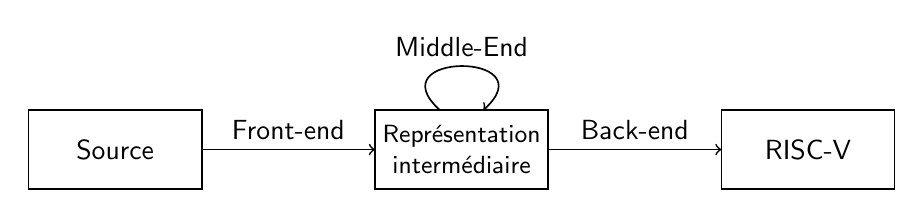
\begin{tikzpicture}[xscale=1.1]
    \draw (0,0) rectangle node {Source} ++(2,1);
    \draw (4,0) rectangle node[align=center,font=\small] {Représentation \\ intermédiaire} ++(2,1);
    \draw (8,0) rectangle node {RISC-V} ++(2,1);

    \draw[->] (2,0.5) -- node[above] {Front-end} ++(2,0);
    \draw[->] (6,0.5) -- node[above] {Back-end} ++(2,0);

    \draw[->] (4.75,1) to[out=135, in=45, distance=30] node[above]
      {Middle-End} ++(0.5,0);
  \end{tikzpicture}
\end{document}
